\section{Experiments}
\label{sec:experiments}

\subsection{Number of Iterations}
One of the major flaws in the graph net framework is the issue of determining how many iterations to run.
In theory, because of the universal approximation properties of neural nets, the optimal number of iterations is any number larger than the diameter of the graph, so that each node can make a fully informed decision knowing the entire graph topology.
However, this is not realistic: as shown in Figure~\ref{fig:dataset-graph-stats}, the maximum diameter of any of the graphs is above 200, meaning that we would have to run the graph neural net for an intractable number of iterations to be able to get the ``full'' result.
Instead, we approximate the result by running fewer iterations, theoretically losing out on certain classes of decisions (although further enforcing our inductive bias, since we believe that local nodes should be the primary ones that matter).
It is not immediately clear how we should choose the \textsc{NIter} hyperparameter though: since graph nets give no formal guarantees that the results monotonically improve with the number of iterations, we have to select the number of iterations through some hyperparameter search.
We ran two experiments to try to select the ideal settings: a \emph{Bayesian Optimization} based approach, and what we call an \emph{Iteration Ensemble} approach.

\begin{figure}
  \centering
  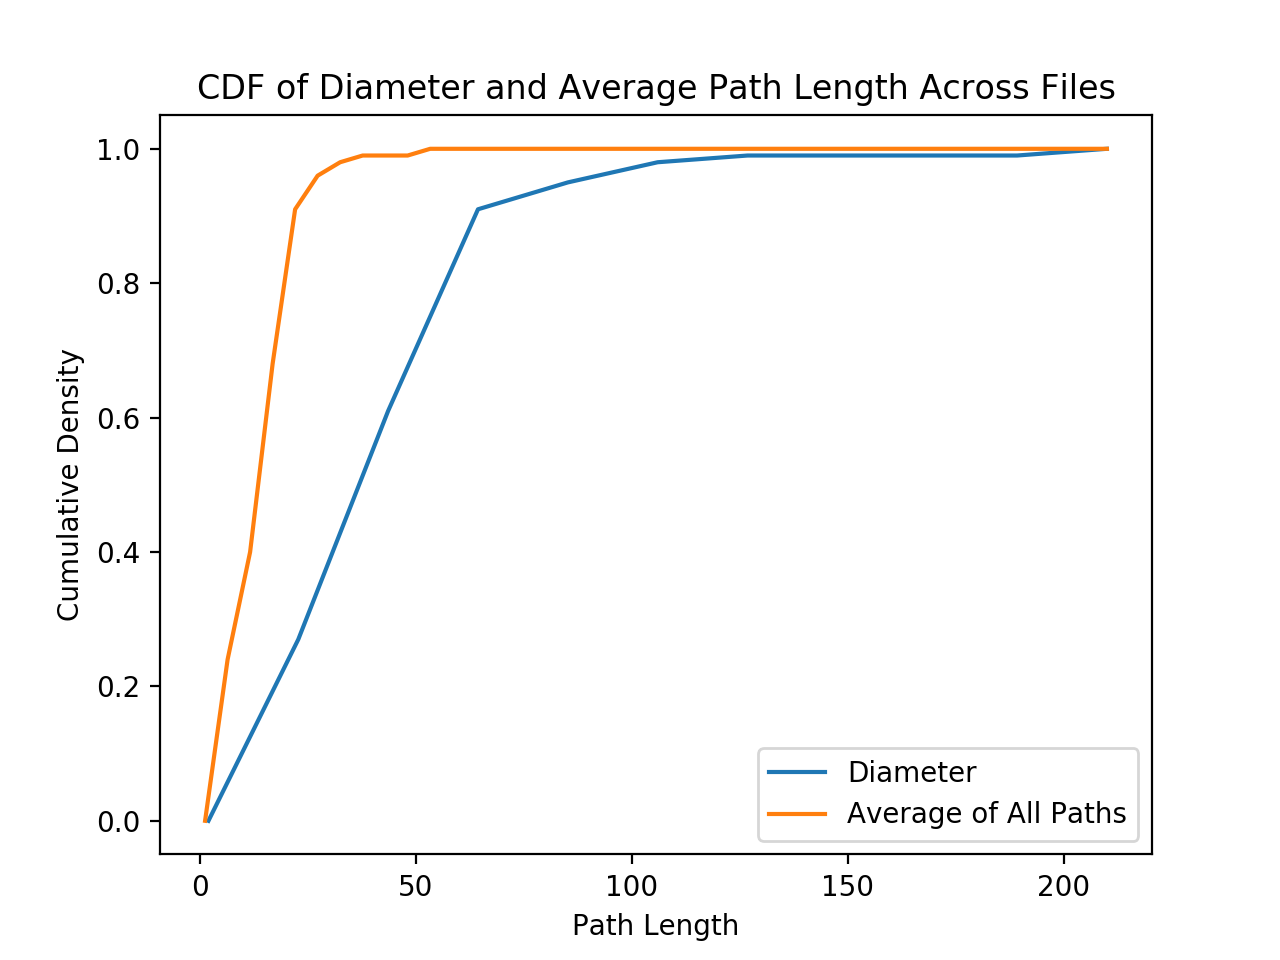
\includegraphics[width=0.49\linewidth]{img/diameter}
  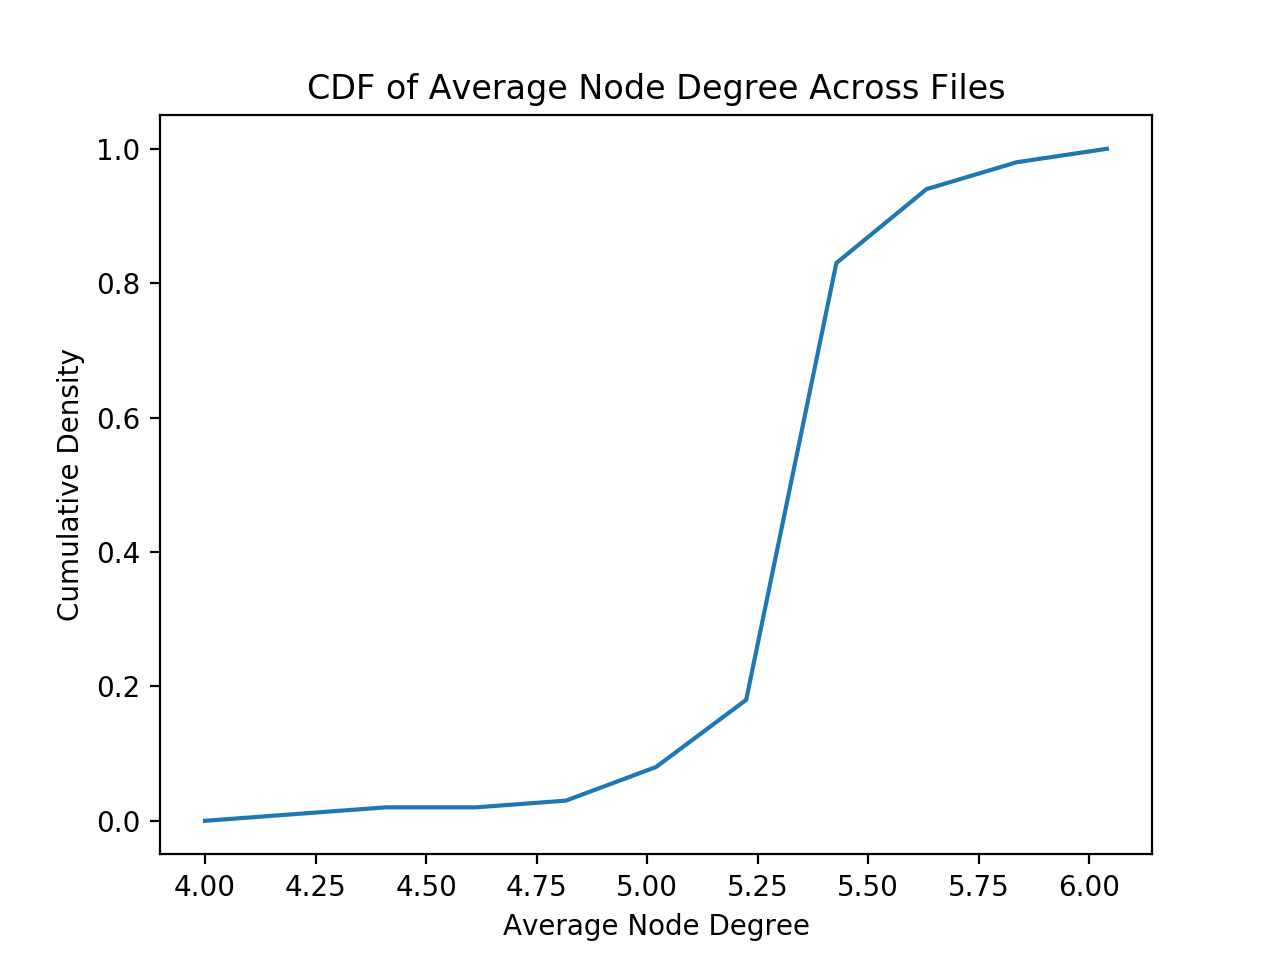
\includegraphics[width=0.49\linewidth]{img/node_degree}
  \caption{Generated graph statistics}
  \label{fig:dataset-graph-stats}
\end{figure}

\paragraph{Bayesian Optimization.}
Our first attempt at finding the ideal number of iterations was inspired by standard approaches to hyperparameter search problems, for cases where running experiments can be prohibitively expensive (the memory and time costs of training a model means we can only search through a relatively small number of possible hyperparameters).
In particular we were inspired by \cite{snoek2012practical}, which suggests using a Bayesian Optimization based approach with an underlying Gaussian Process to pick hyperparameters, using the expected improvement metric (expectation of the decrease in the desired metric over the current best known hyperparameter) to explore the hyperparameter space.
The metric we chose to optimize over was the train loss after 3 epochs.
Selecting the best performing number of iterations in this metric gave us confidence that the network had actually made progress in learning significant features of the dataset, while also being sure not to overfit to our validation set.
The results of this experiment can be seen in Figure~\ref{fig:gp-diagram}, which shows the confidence bounds on the number of iterations to use in the range $[0, 10]$, which gave us a satisfactory coverage of the average path length seen in Figure~\ref{fig:dataset-graph-stats}, while still being computationally tractable to train.
\todo{what parameter did this say we should use}

\paragraph{Iteration Ensemble.}
Our second attempt at hyperparameter search followed a more optimization based approach.
Rather than trying to pick one specific ideal number of iterations, we ran an ensemble over several choices of iteration counts, using a learned weighting to linearly combine all of their predictions in the last step to produce the final result.
Importantly, we ran this iteration ensemble on \emph{one single graph net}; that is, we combined each of the intermediate predictions of running a single graph neural net.
We took this approach for two reasons: primarily, it was more computationally efficient (running large ensembles of graph nets was not possible on the machines we had access to), but it also enforced one of the inductive biases we hoped to see in a solution: intermediate steps of the graph net message passing algorithm should roughly correspond to finer and finer approximations of the posterior prediction, meaning all steps should be valid (if unrefined) predictions.
We also hoped to see situations where some weights on the upper or lower end would drop away, signifying that we should shift the number of iterations that comprise the ensemble.

Ultimately, this did not work as well as we hoped, and our best results were achieved by just using a single number of iterations learned through the Bayesian Optimization approach.
The linear combination weight vector changed only marginally from its initial value, and the prediction quality was no better than that of using a fixed number of iterations.
We believe this happened for one primary reason: one or two iterations were good enough, as shown by the Bayesian Optimization approach.
Any iterations beyond that did not refine the search, and since we did not penalize their existence through any regularization (only the wrongness of their predictions), they stayed around as unnecessary artifacts that did not get pruned.


\subsection{Edge Ablation}
To determine whether our graph structure (nodes and edges) was chosen correctly, we performed a set of ablation studies.
Specifically, we ran experiments using the optimally chosen hyperparameters where we entirely deleted each class of edges (AST edges, Token edges, and Variable edges) from the graph, and compared performance to the original.
The results of these studies can be seen in Table~\ref{table:results}.
\todo{does this validate our construction? say we went over the top? TBD!}


%%% Local Variables:
%%% TeX-master: "main"
%%% End: